 \begin{figure}[htbp]
  \centering
  \begin{tabular}{cccc}
    \subfloat[]{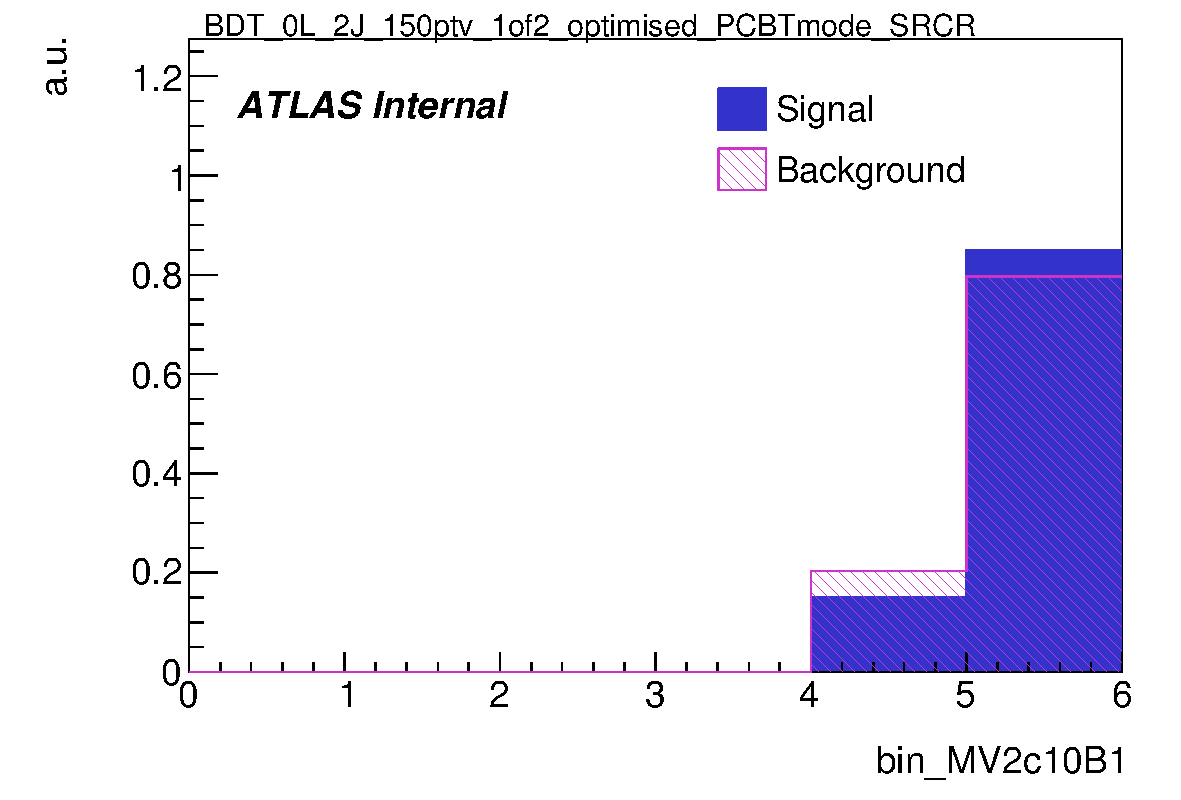
\includegraphics[width=0.33\linewidth]{0-lep-mva/Distr_SignalBackground_bin_MV2c10B1_BDT_0L_2J_150ptv_1of2_optimised_PCBTmode_SRCR-eps-converted-to}}
    \subfloat[]{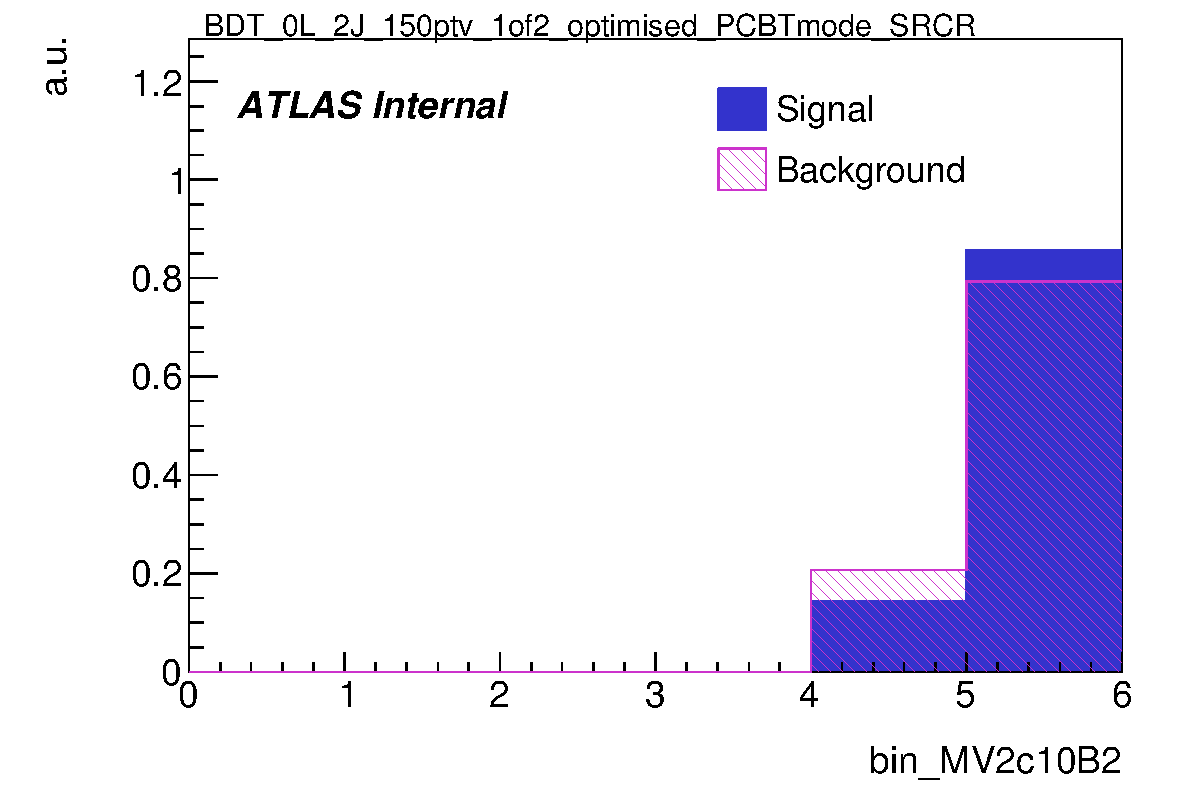
\includegraphics[width=0.33\linewidth]{0-lep-mva/Distr_SignalBackground_bin_MV2c10B2_BDT_0L_2J_150ptv_1of2_optimised_PCBTmode_SRCR-eps-converted-to}}
     \subfloat[]{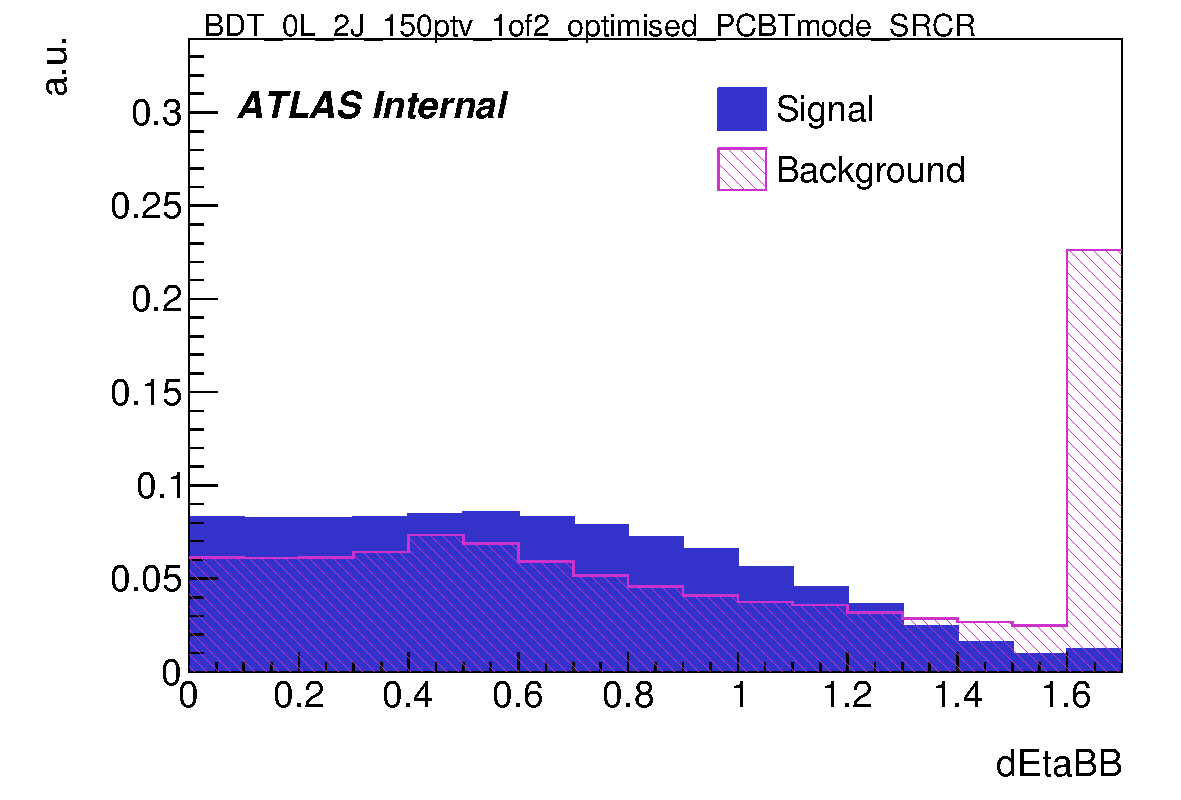
\includegraphics[width=0.33\linewidth]{0-lep-mva/Distr_SignalBackground_dEtaBB_BDT_0L_2J_150ptv_1of2_optimised_PCBTmode_SRCR-eps-converted-to}}\\
    \subfloat[]{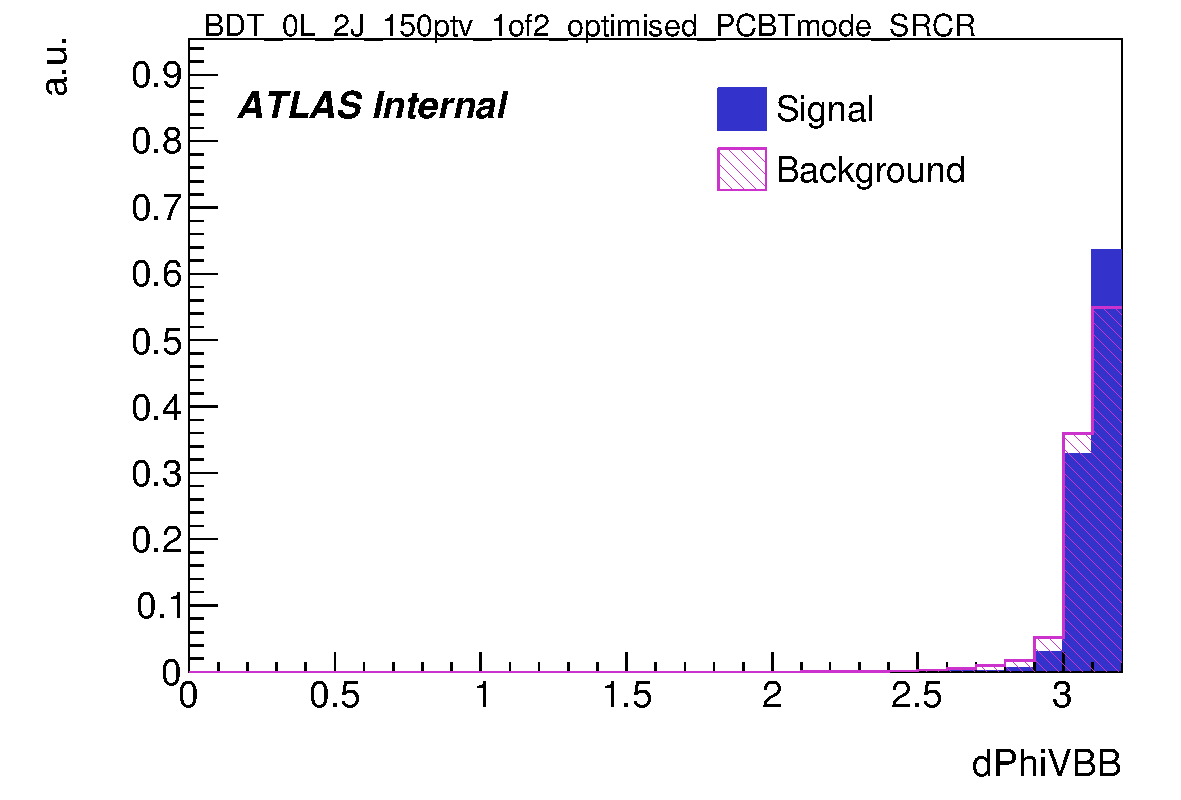
\includegraphics[width=0.33\linewidth]{0-lep-mva/Distr_SignalBackground_dPhiVBB_BDT_0L_2J_150ptv_1of2_optimised_PCBTmode_SRCR-eps-converted-to}}
    \subfloat[]{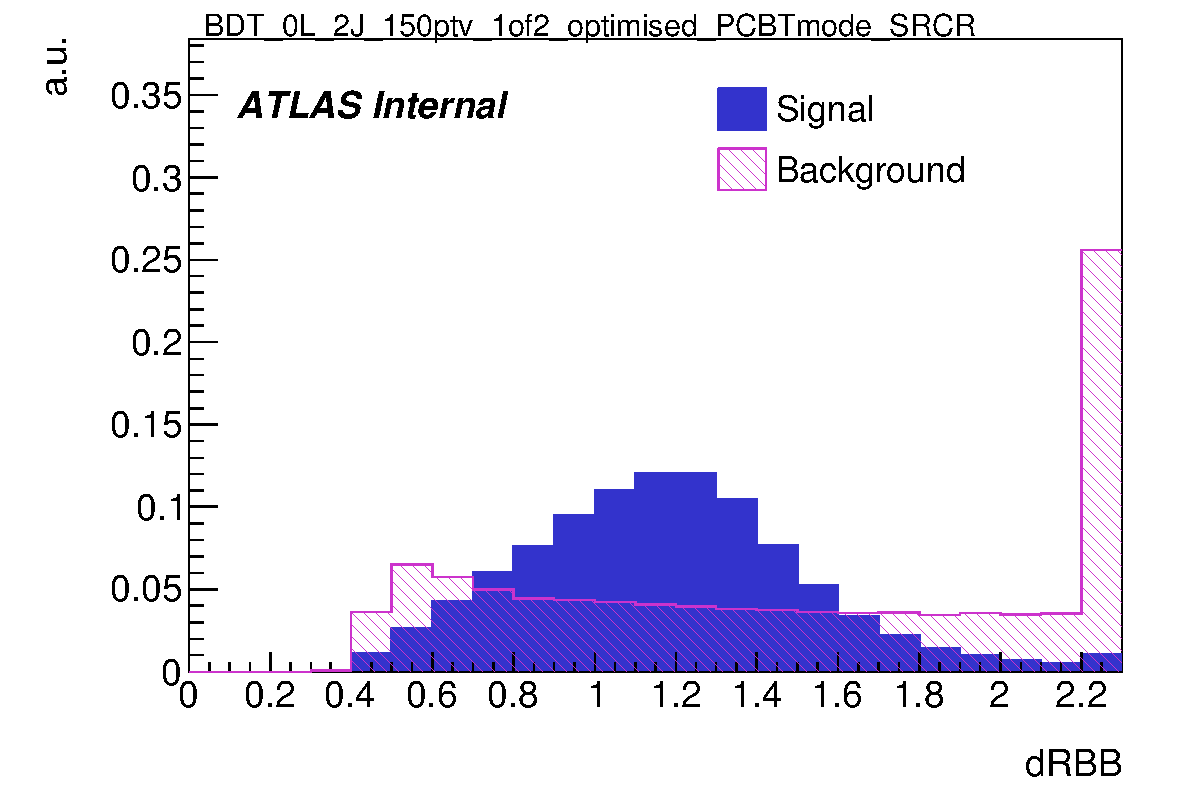
\includegraphics[width=0.33\linewidth]{0-lep-mva/Distr_SignalBackground_dRBB_BDT_0L_2J_150ptv_1of2_optimised_PCBTmode_SRCR-eps-converted-to}}
     \subfloat[]{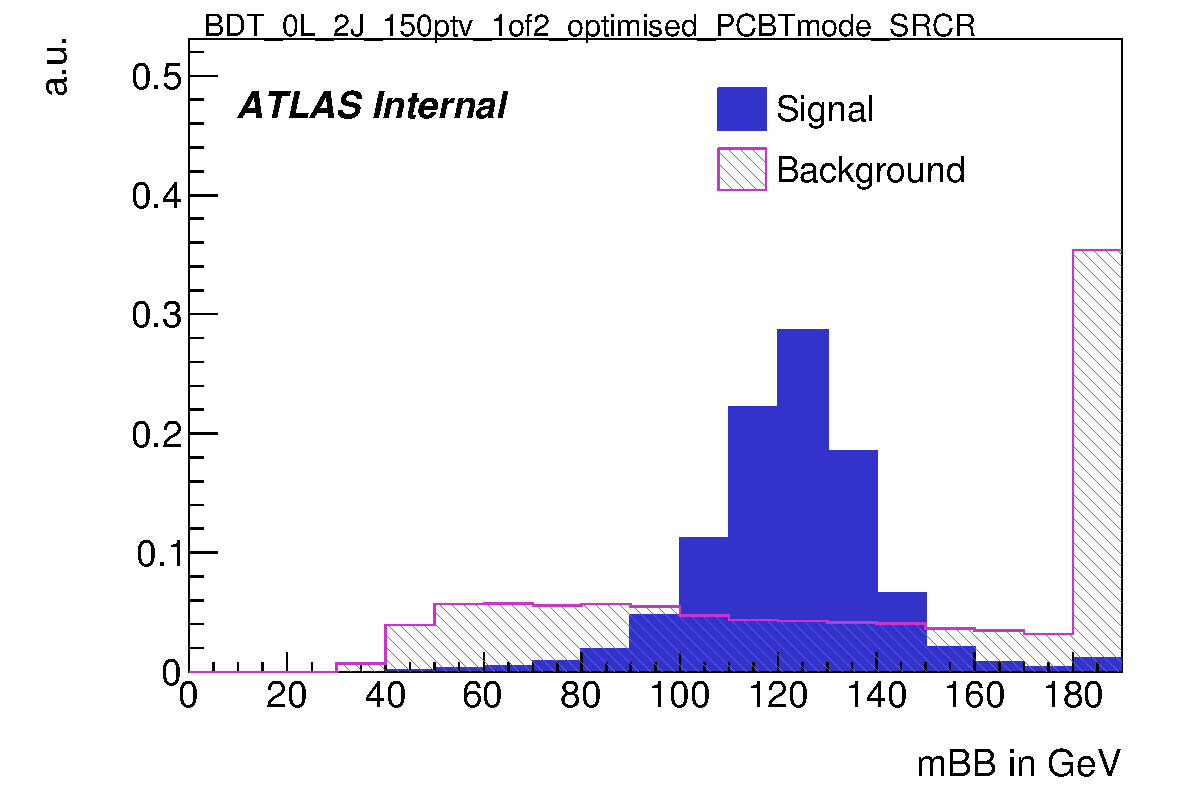
\includegraphics[width=0.33\linewidth]{0-lep-mva/Distr_SignalBackground_mBB_BDT_0L_2J_150ptv_1of2_optimised_PCBTmode_SRCR-eps-converted-to}}\\
    \subfloat[]{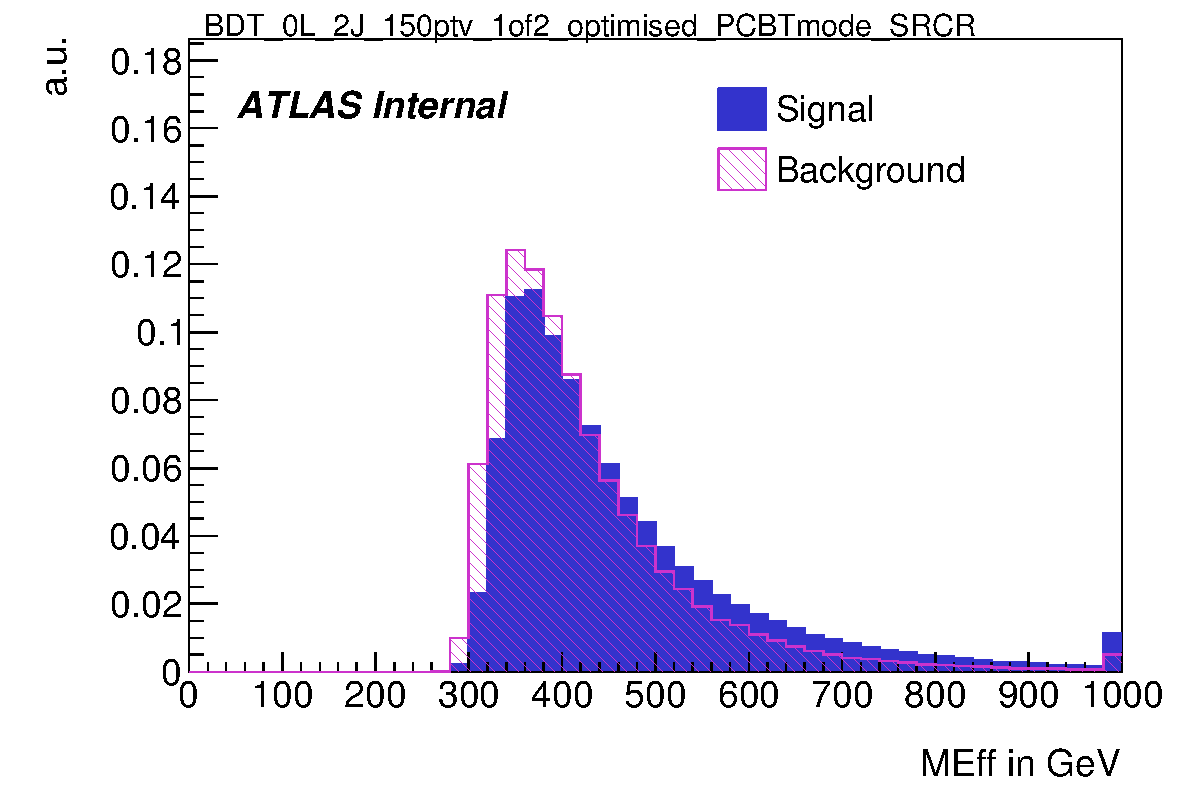
\includegraphics[width=0.33\linewidth]{0-lep-mva/Distr_SignalBackground_MEff_BDT_0L_2J_150ptv_1of2_optimised_PCBTmode_SRCR-eps-converted-to}}
     \subfloat[]{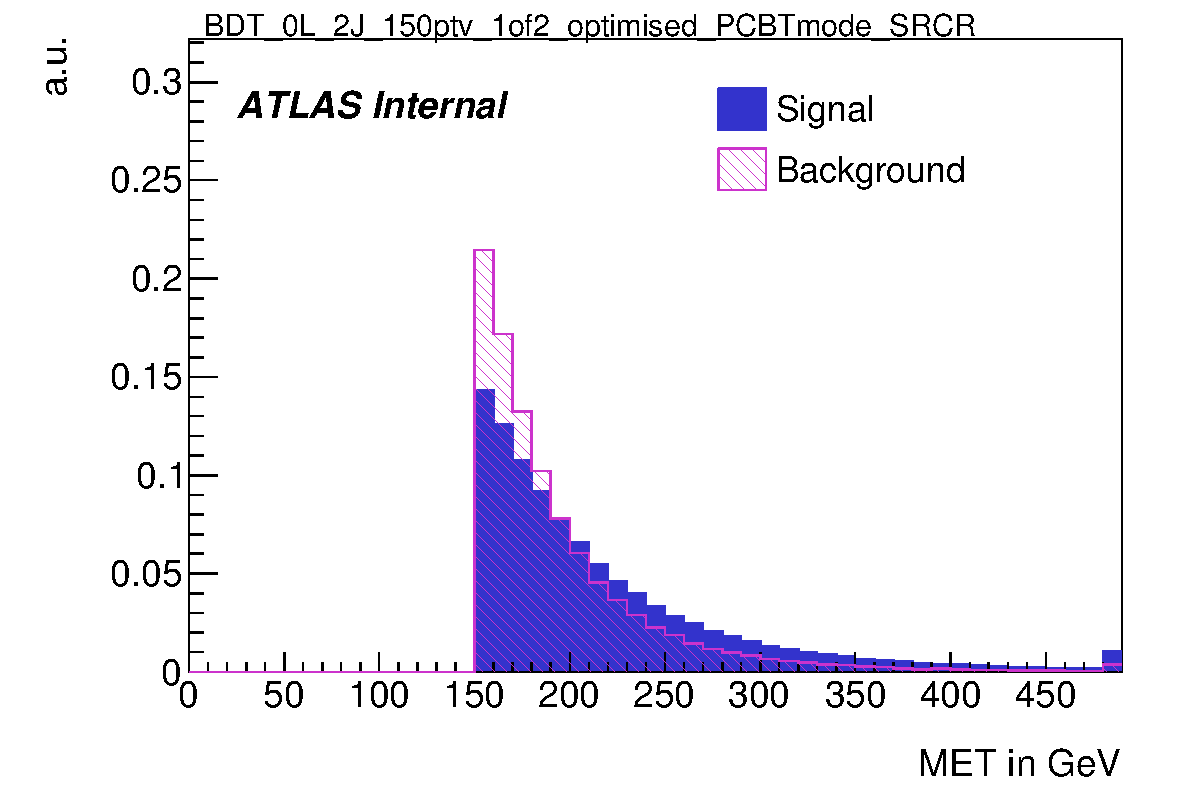
\includegraphics[width=0.33\linewidth]{0-lep-mva/Distr_SignalBackground_MET_BDT_0L_2J_150ptv_1of2_optimised_PCBTmode_SRCR-eps-converted-to}}          
    \subfloat[]{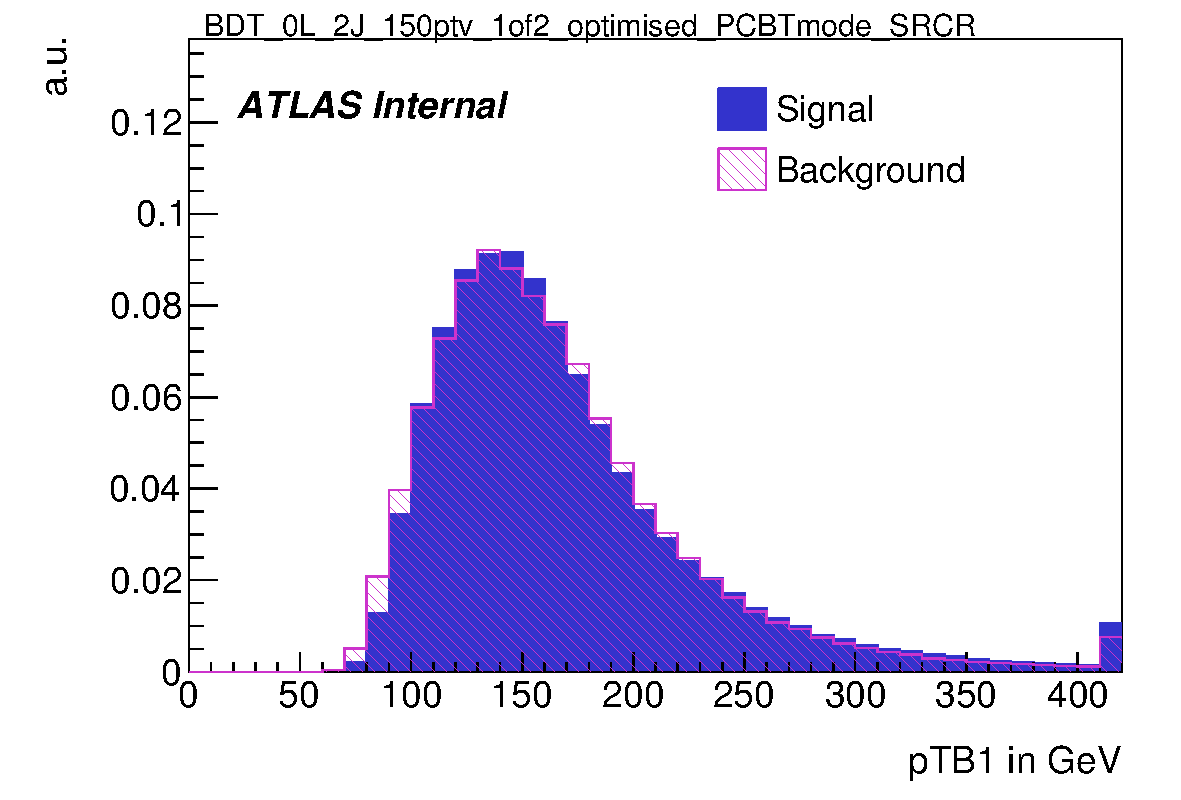
\includegraphics[width=0.33\linewidth]{0-lep-mva/Distr_SignalBackground_pTB1_BDT_0L_2J_150ptv_1of2_optimised_PCBTmode_SRCR-eps-converted-to}} \\
    \subfloat[]{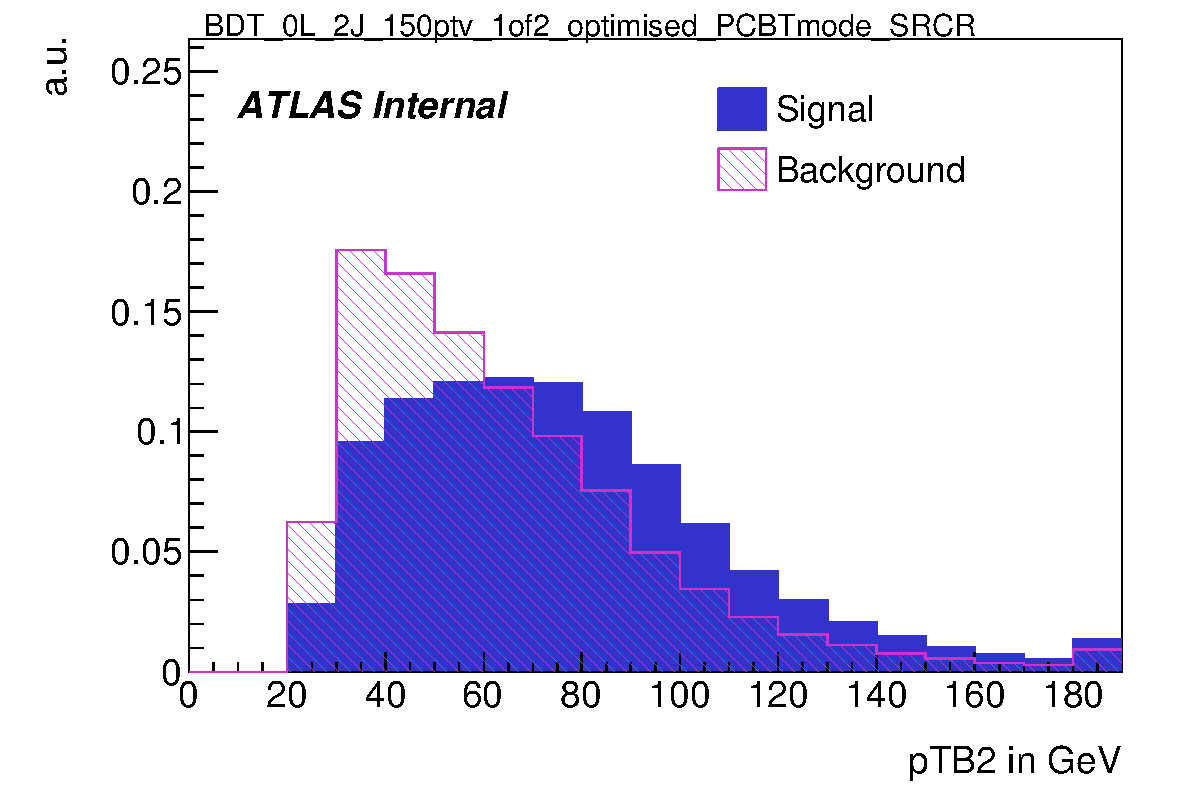
\includegraphics[width=0.33\linewidth]{0-lep-mva/Distr_SignalBackground_pTB2_BDT_0L_2J_150ptv_1of2_optimised_PCBTmode_SRCR-eps-converted-to}}   
    \subfloat[]{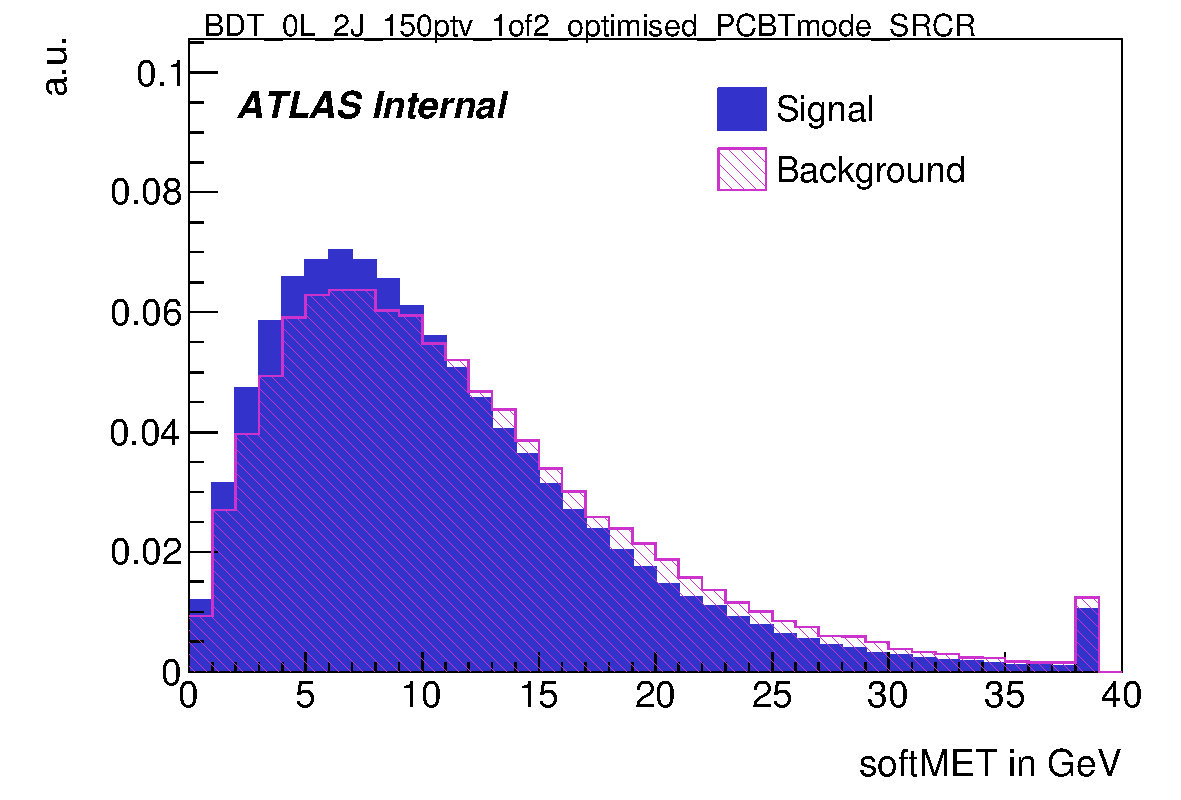
\includegraphics[width=0.33\linewidth]{0-lep-mva/Distr_SignalBackground_softMET_BDT_0L_2J_150ptv_1of2_optimised_PCBTmode_SRCR-eps-converted-to}}\\    
    \end{tabular}
    \caption[Inputs to the multi-variate analysis in the 0--lepton 2--jet
    region.]{Inputs to the multi-variate analysis in the 0--lepton 2--jet
      region. Signal events are shown in blue and background events are shown in
      red. The signal and background histograms have been normalised to the same
      area. The distributions only include events with $E_{\mathrm{T}}^{\text{miss}}$ > 150
      \GeV.}
    \label{fig:bdtinputs-0lep}
\end{figure}

 \begin{figure}[htbp]
  \centering
  \begin{tabular}{cccc}
    \subfloat[]{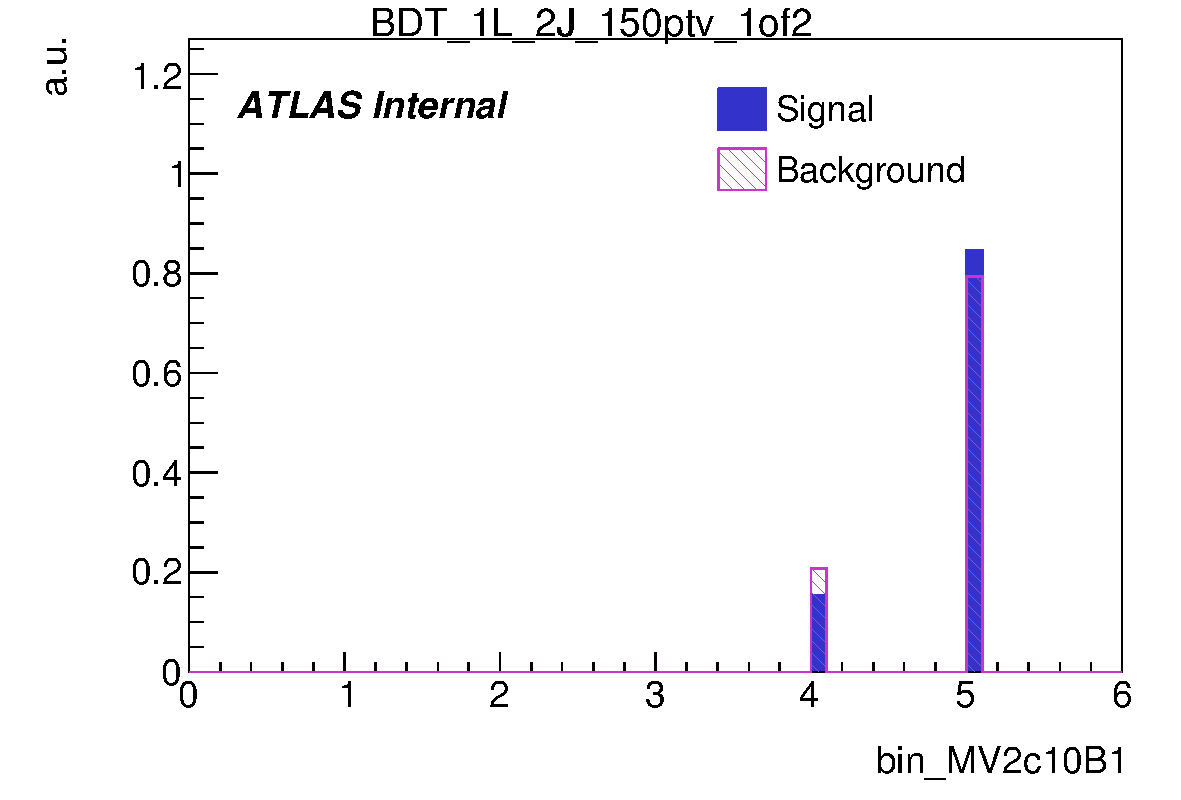
\includegraphics[width=0.3\linewidth]{1-lep-mva/Distr_SignalBackground_bin_MV2c10B1_BDT_1L_2J_150ptv_1of2-eps-converted-to}}
    \subfloat[]{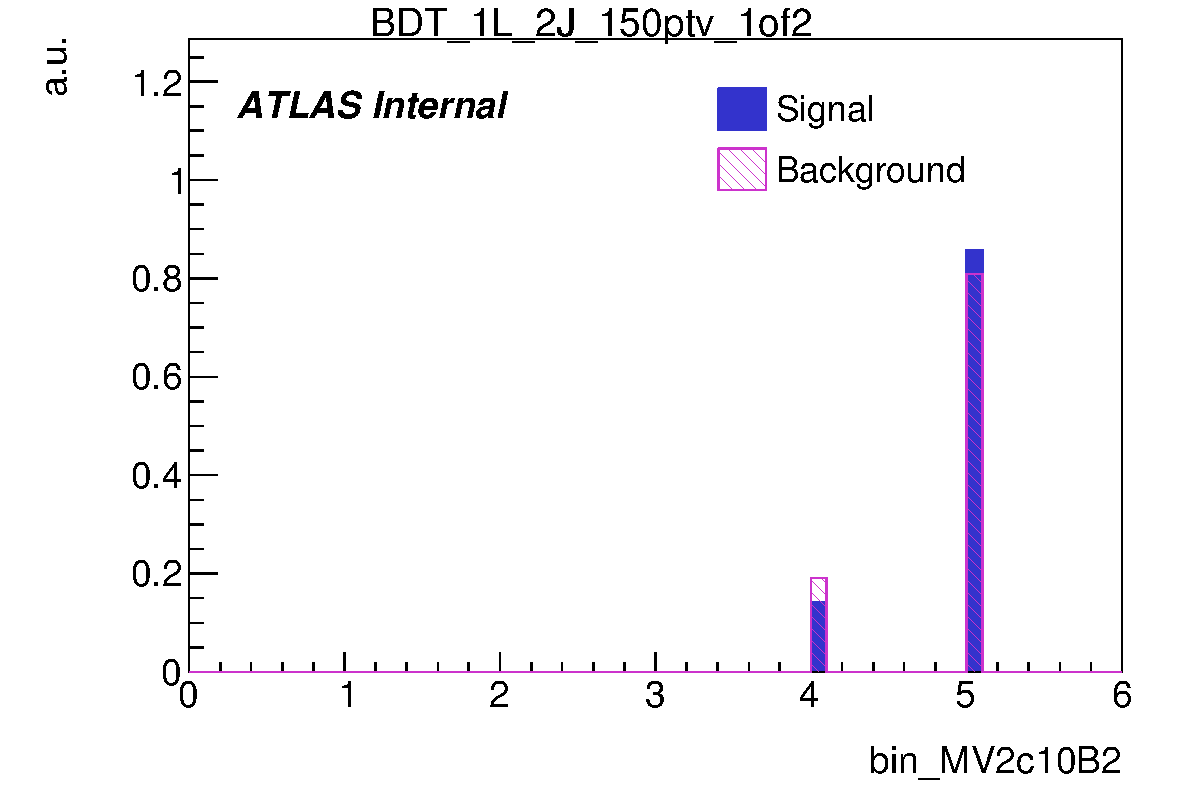
\includegraphics[width=0.3\linewidth]{1-lep-mva/Distr_SignalBackground_bin_MV2c10B2_BDT_1L_2J_150ptv_1of2-eps-converted-to}}
     \subfloat[]{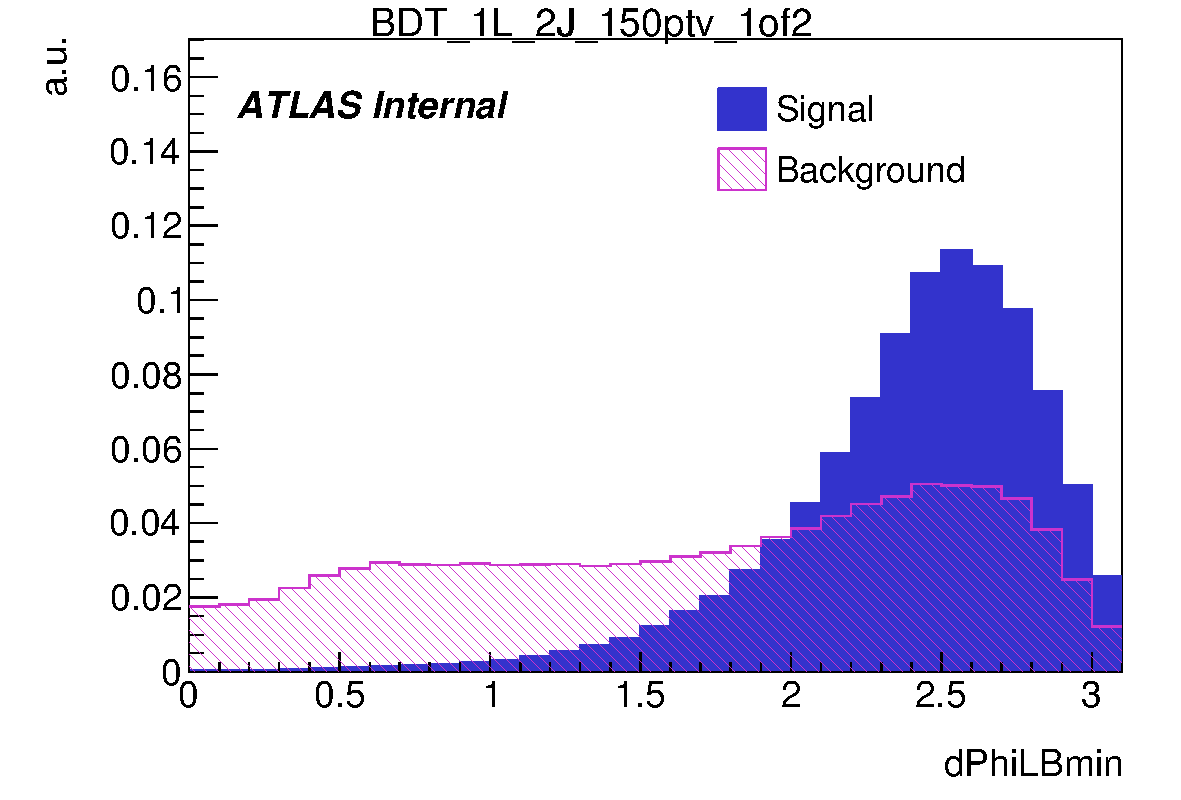
\includegraphics[width=0.3\linewidth]{1-lep-mva/Distr_SignalBackground_dPhiLBmin_BDT_1L_2J_150ptv_1of2-eps-converted-to}}\\
    \subfloat[]{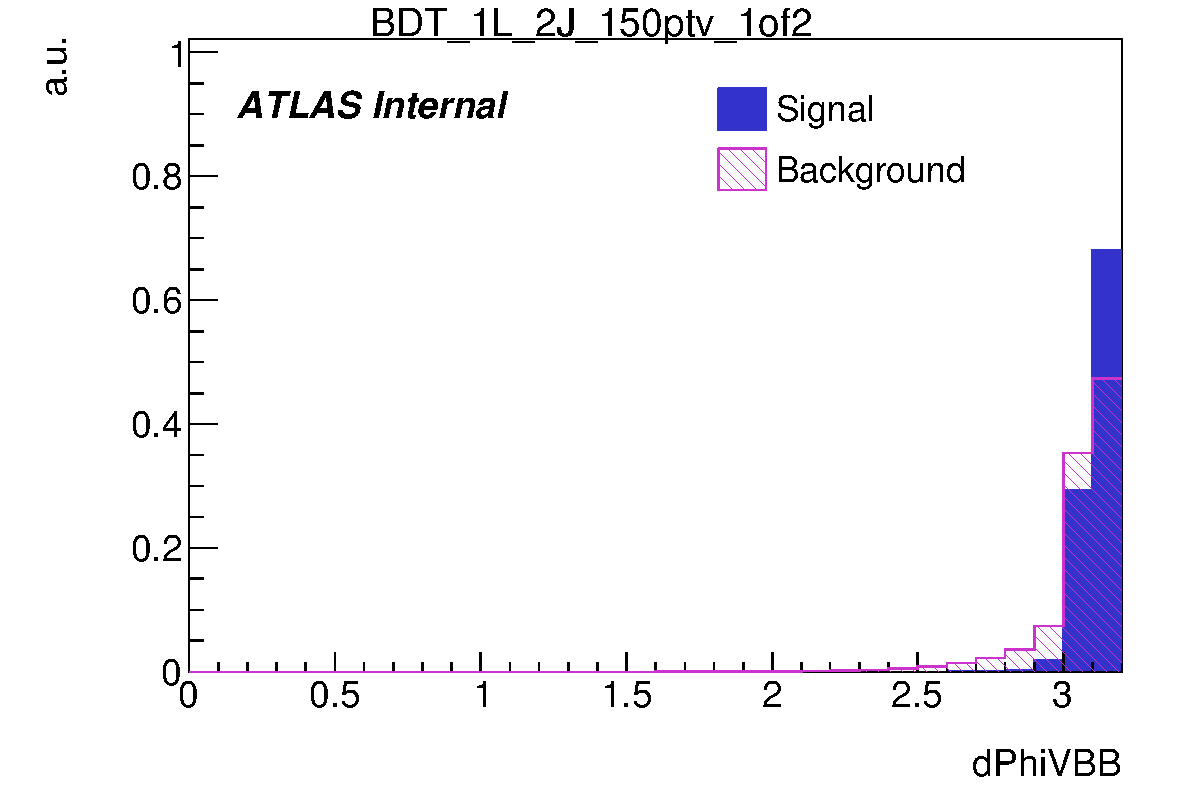
\includegraphics[width=0.3\linewidth]{1-lep-mva/Distr_SignalBackground_dPhiVBB_BDT_1L_2J_150ptv_1of2-eps-converted-to}}
    \subfloat[]{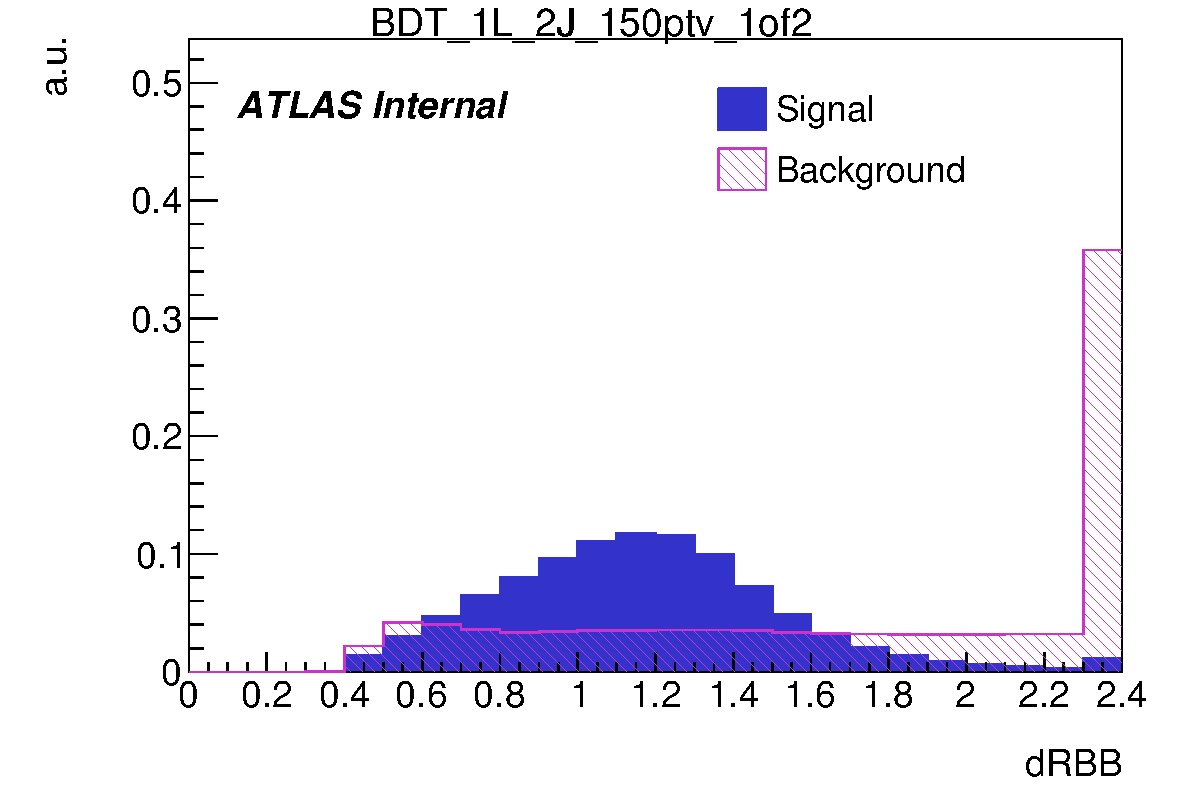
\includegraphics[width=0.3\linewidth]{1-lep-mva/Distr_SignalBackground_dRBB_BDT_1L_2J_150ptv_1of2-eps-converted-to}}
     \subfloat[]{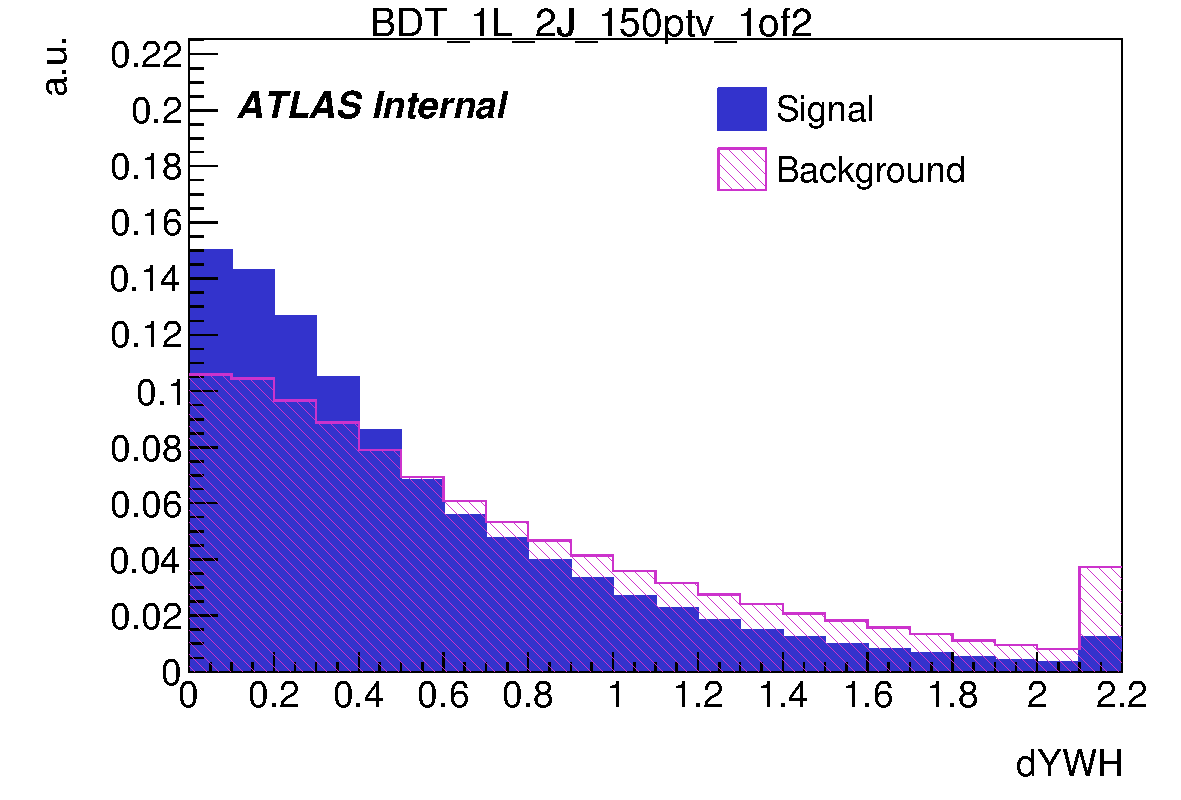
\includegraphics[width=0.3\linewidth]{1-lep-mva/Distr_SignalBackground_dYWH_BDT_1L_2J_150ptv_1of2-eps-converted-to}}\\
    \subfloat[]{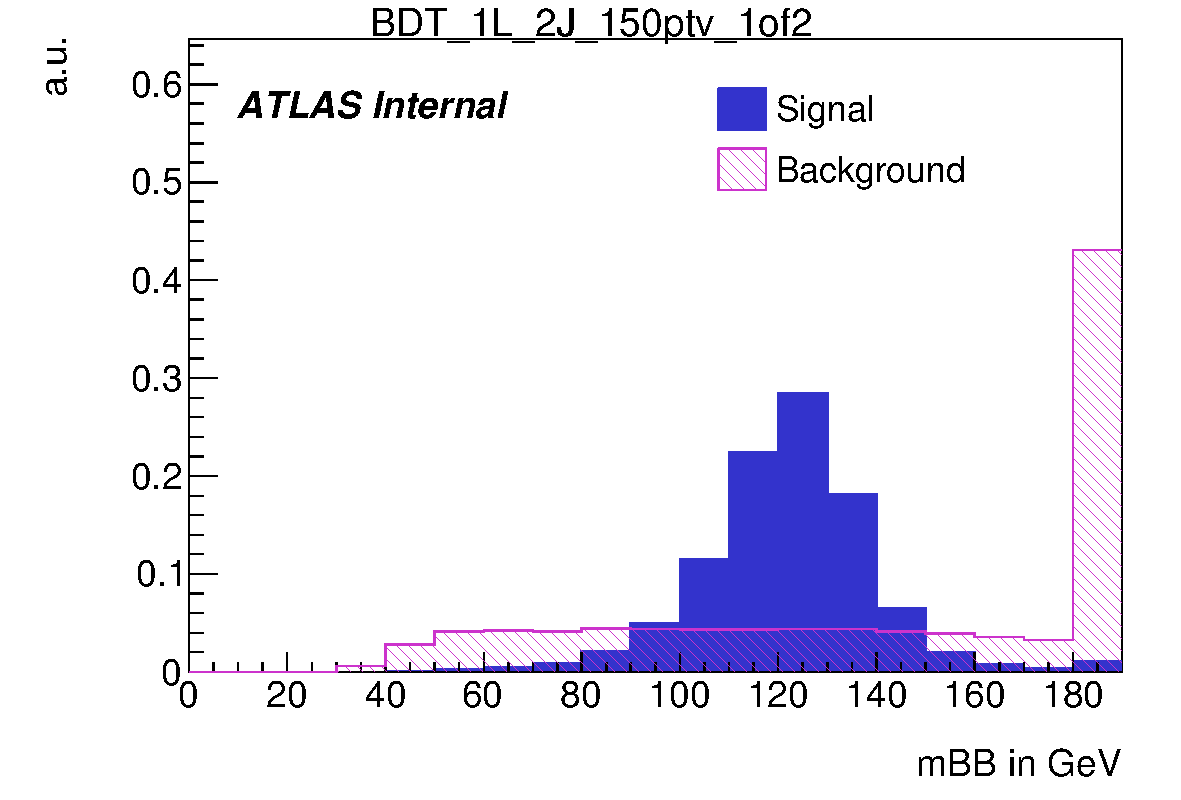
\includegraphics[width=0.3\linewidth]{1-lep-mva/Distr_SignalBackground_mBB_BDT_1L_2J_150ptv_1of2-eps-converted-to}}
     \subfloat[]{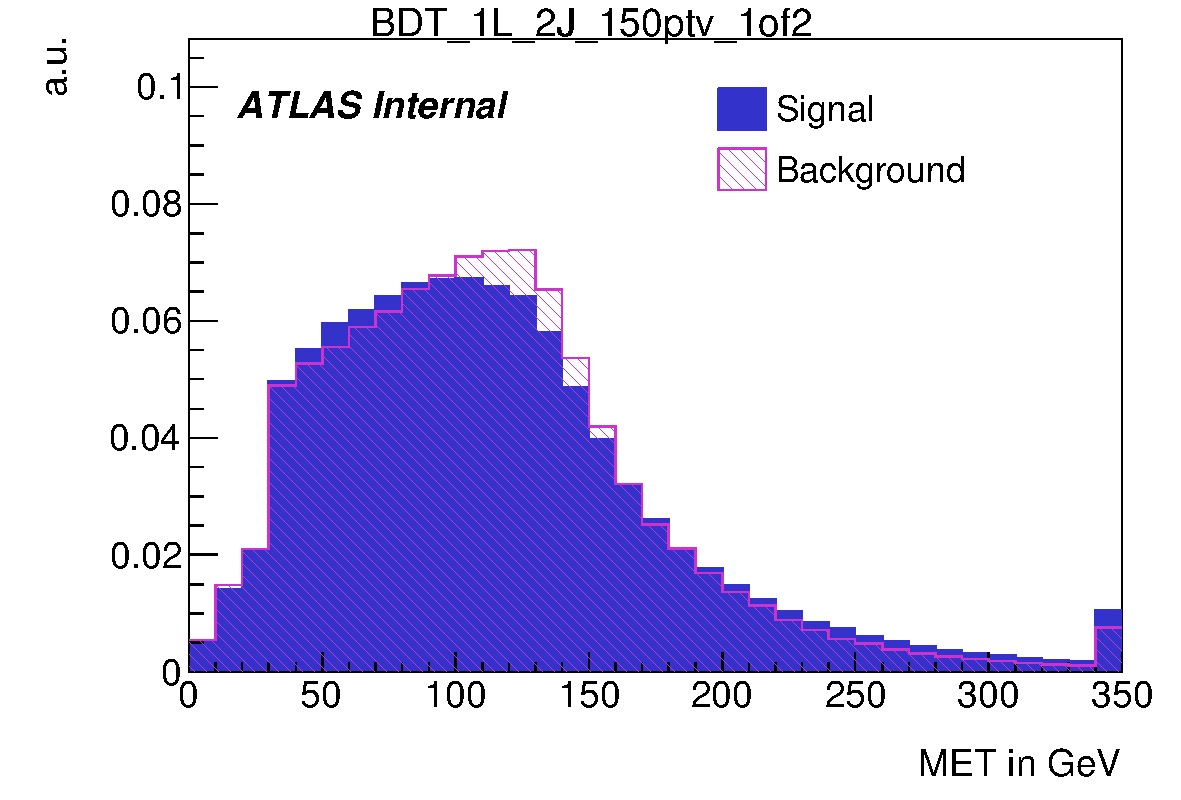
\includegraphics[width=0.3\linewidth]{1-lep-mva/Distr_SignalBackground_MET_BDT_1L_2J_150ptv_1of2-eps-converted-to}}          
    \subfloat[]{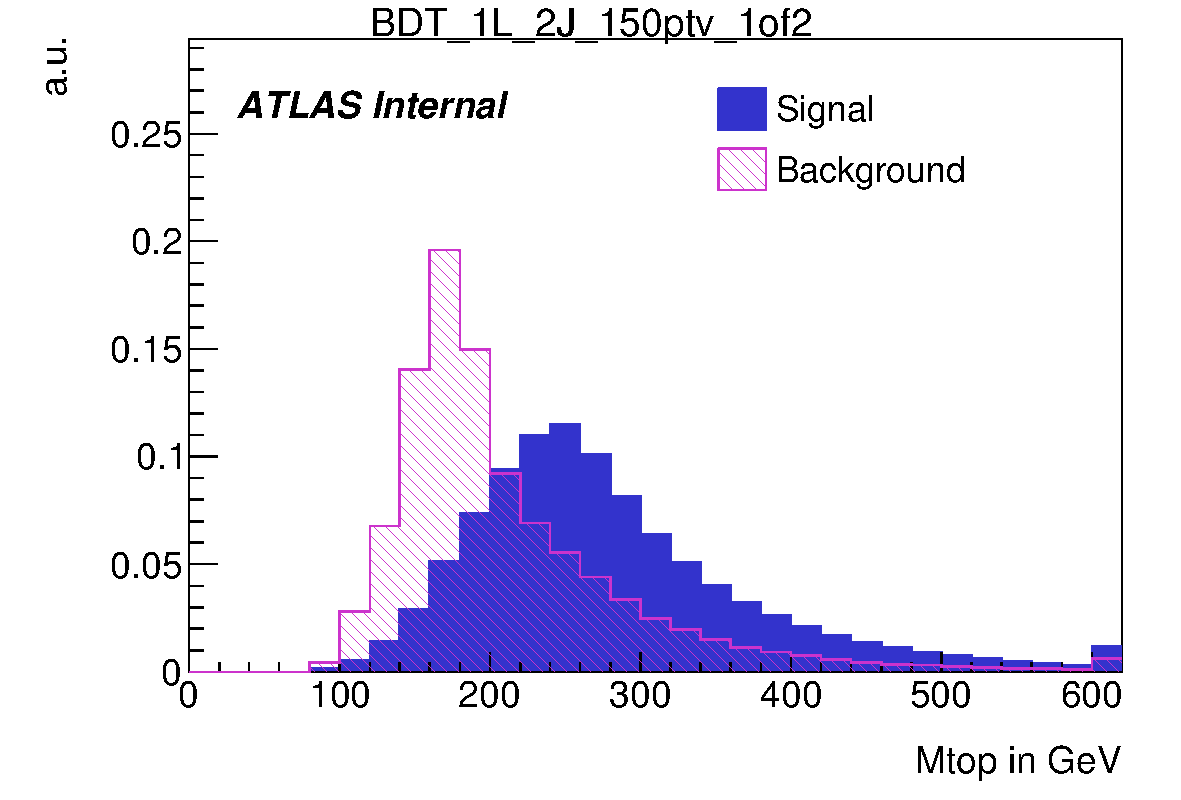
\includegraphics[width=0.3\linewidth]{1-lep-mva/Distr_SignalBackground_Mtop_BDT_1L_2J_150ptv_1of2-eps-converted-to}} \\
    \subfloat[]{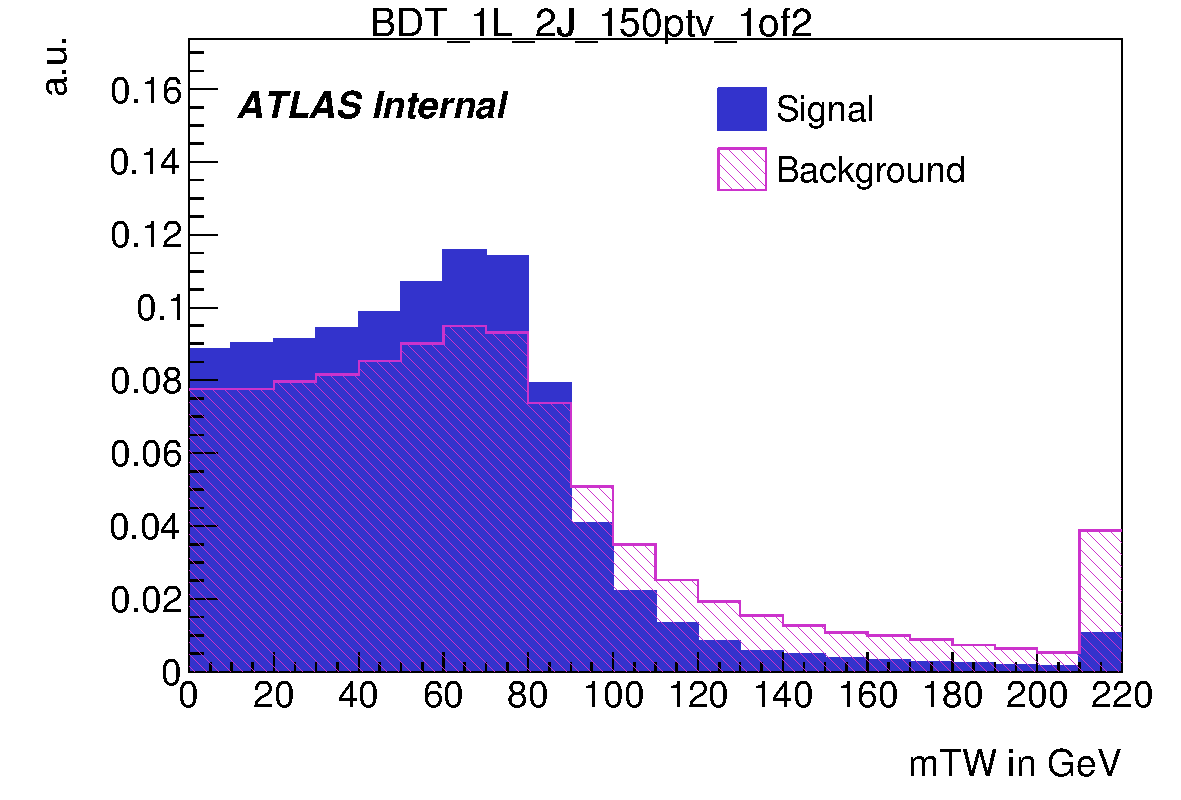
\includegraphics[width=0.3\linewidth]{1-lep-mva/Distr_SignalBackground_mTW_BDT_1L_2J_150ptv_1of2-eps-converted-to}}   
    \subfloat[]{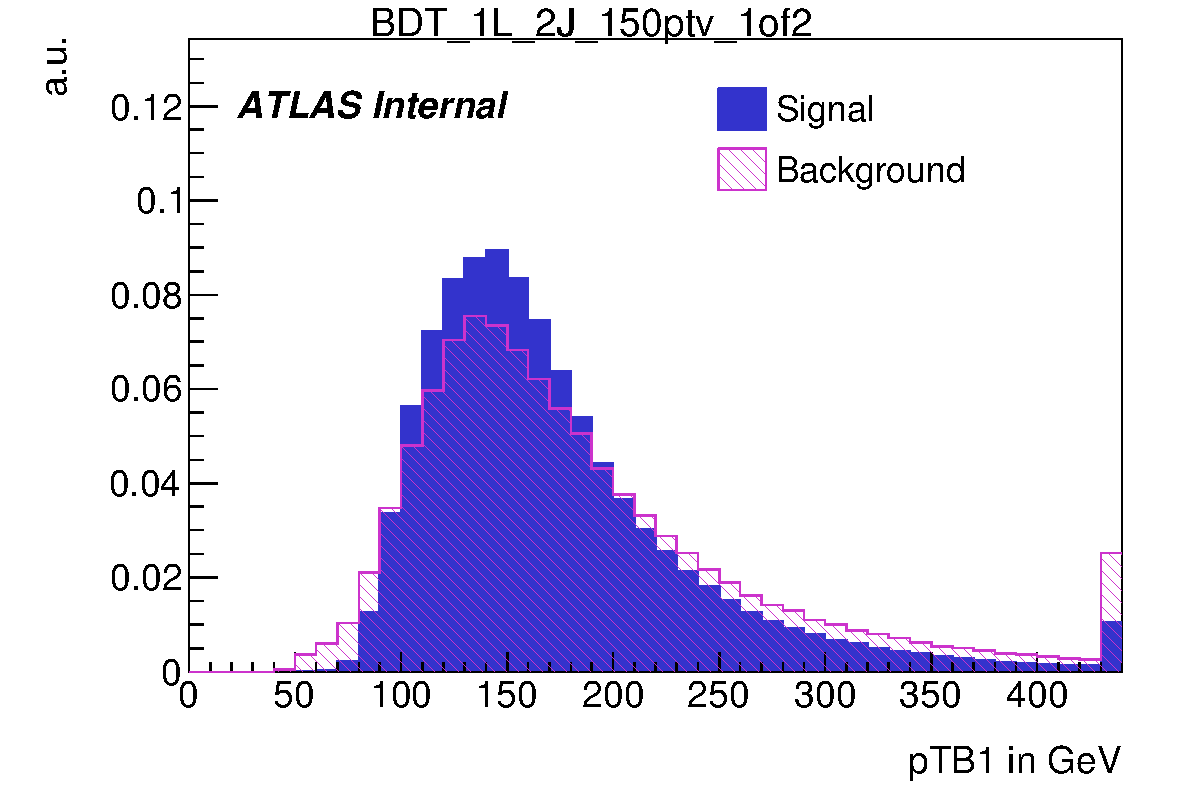
\includegraphics[width=0.3\linewidth]{1-lep-mva/Distr_SignalBackground_pTB1_BDT_1L_2J_150ptv_1of2-eps-converted-to}}
    \subfloat[]{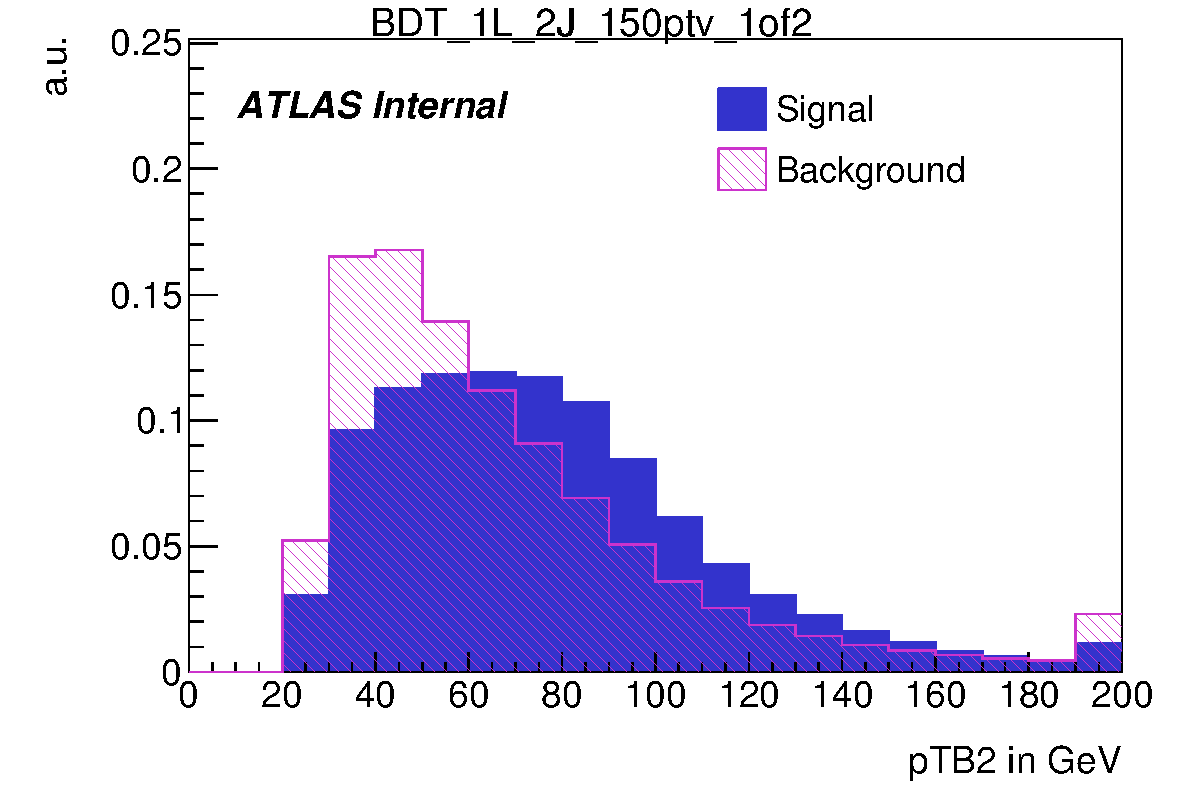
\includegraphics[width=0.3\linewidth]{1-lep-mva/Distr_SignalBackground_pTB2_BDT_1L_2J_150ptv_1of2-eps-converted-to}}\\   
    \subfloat[]{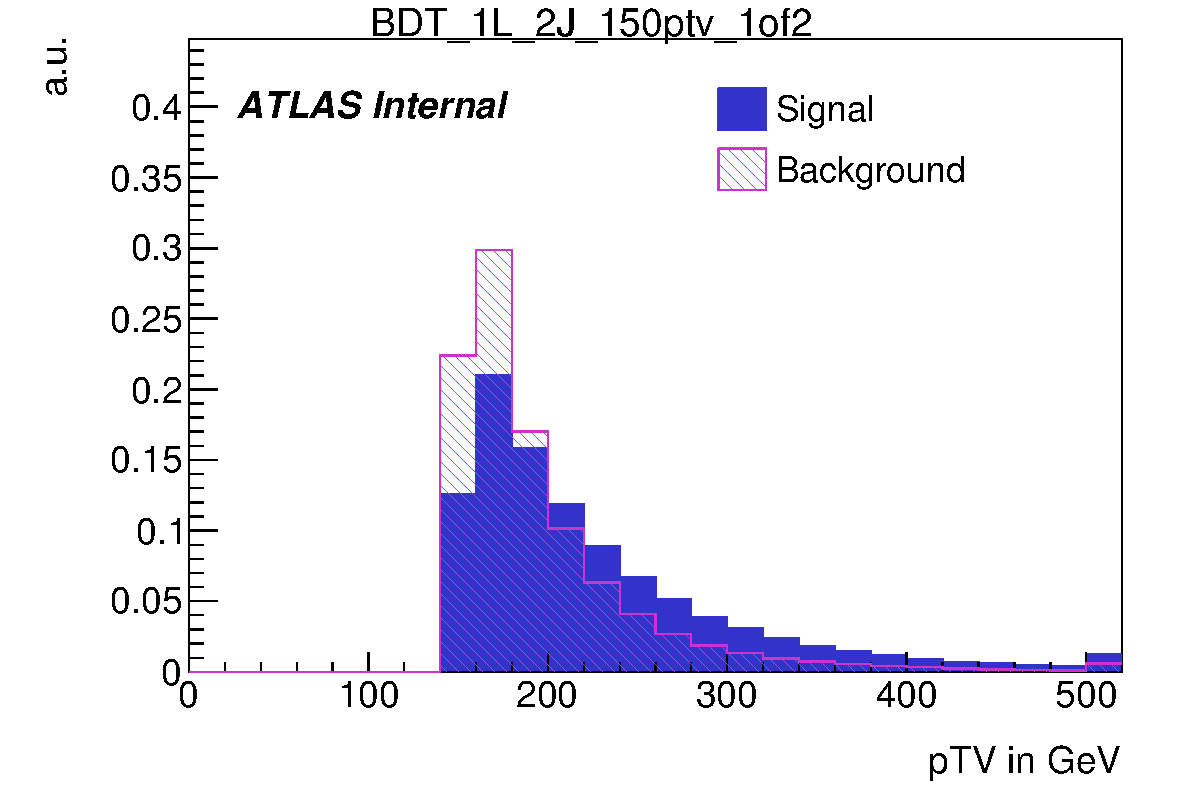
\includegraphics[width=0.3\linewidth]{1-lep-mva/Distr_SignalBackground_pTV_BDT_1L_2J_150ptv_1of2-eps-converted-to}} 
    \end{tabular}
    \caption[Inputs to the multi-variate analysis in the 1--lepton 2--jet
    region.]{Inputs to the multi-variate analysis in the 1--lepton 2--jet
      region. Signal events are shown in blue and background events are shown in
      red. The signal and background histograms have been normalised to the same
      area.The distributions only include events with $p_{\mathrm{T}}^{W}$ > 150
      \GeV.}
    \label{fig:bdtinputs-1lep}
\end{figure}

 \begin{figure}[htbp]
  \centering
  \begin{tabular}{cccc}
    \subfloat[]{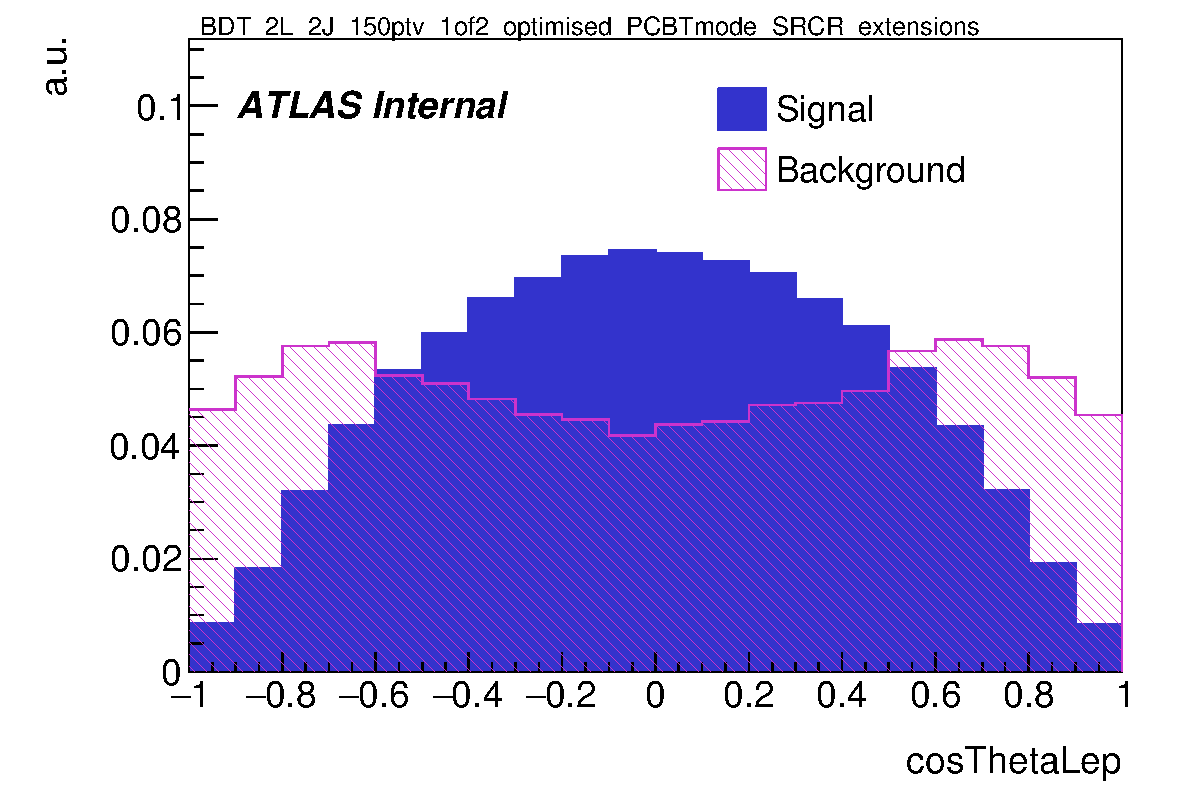
\includegraphics[width=0.33\linewidth]{2-lep-mva/Distr_SignalBackground_cosThetaLep_BDT_2L_2J_150ptv_1of2_optimised_PCBTmode_SRCR_extensions-eps-converted-to}}
    \subfloat[]{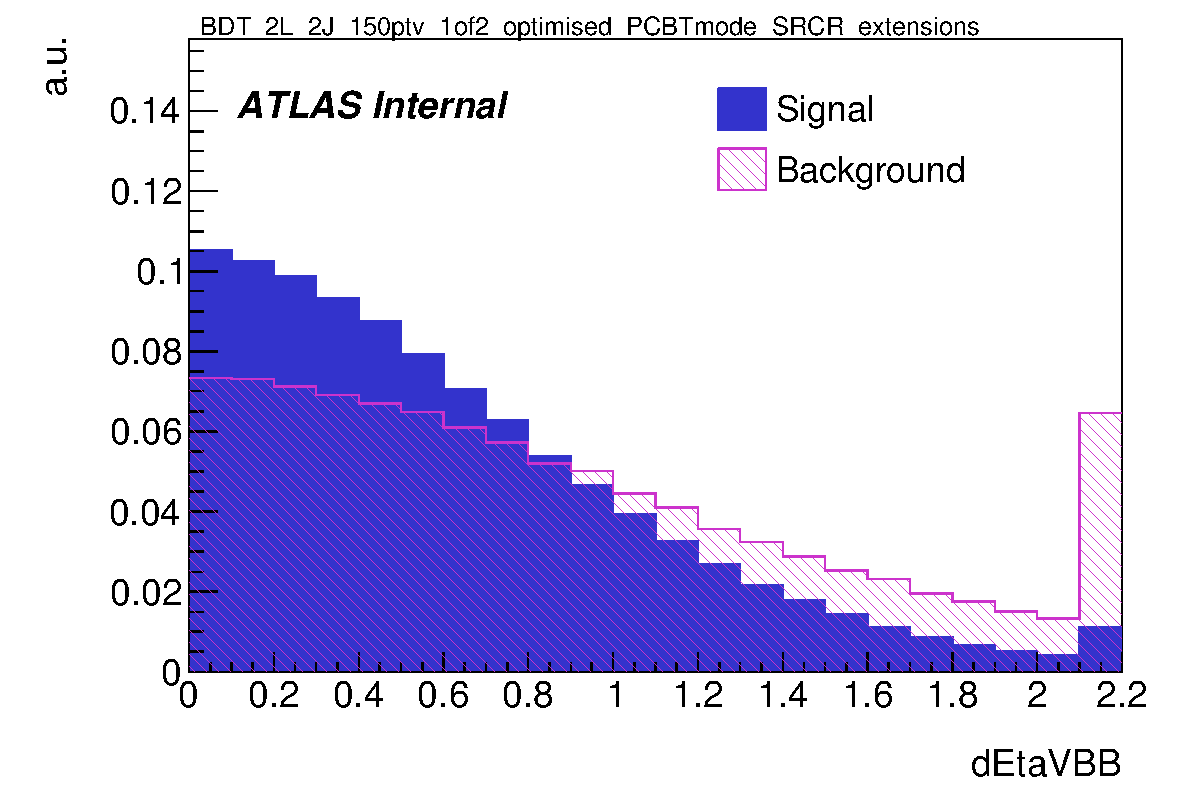
\includegraphics[width=0.33\linewidth]{2-lep-mva/Distr_SignalBackground_dEtaVBB_BDT_2L_2J_150ptv_1of2_optimised_PCBTmode_SRCR_extensions-eps-converted-to}}
     \subfloat[]{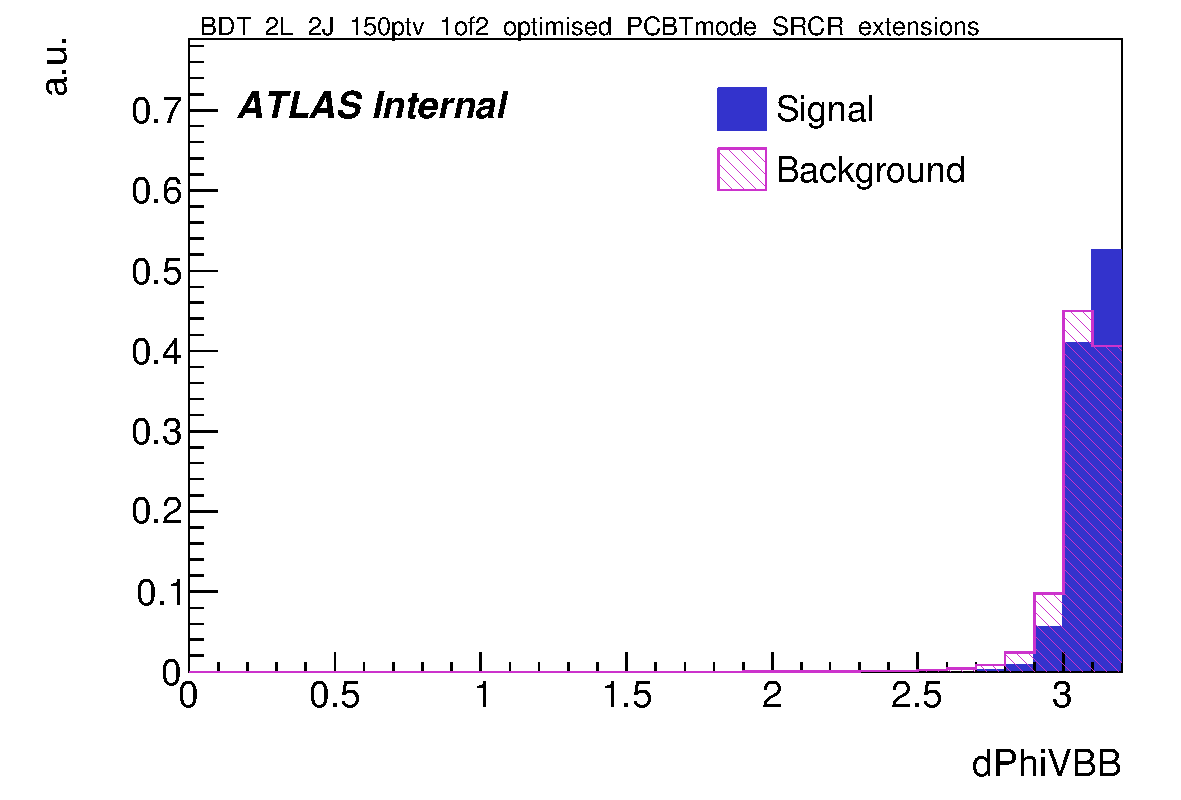
\includegraphics[width=0.33\linewidth]{2-lep-mva/Distr_SignalBackground_dPhiVBB_BDT_2L_2J_150ptv_1of2_optimised_PCBTmode_SRCR_extensions-eps-converted-to}}\\
    \subfloat[]{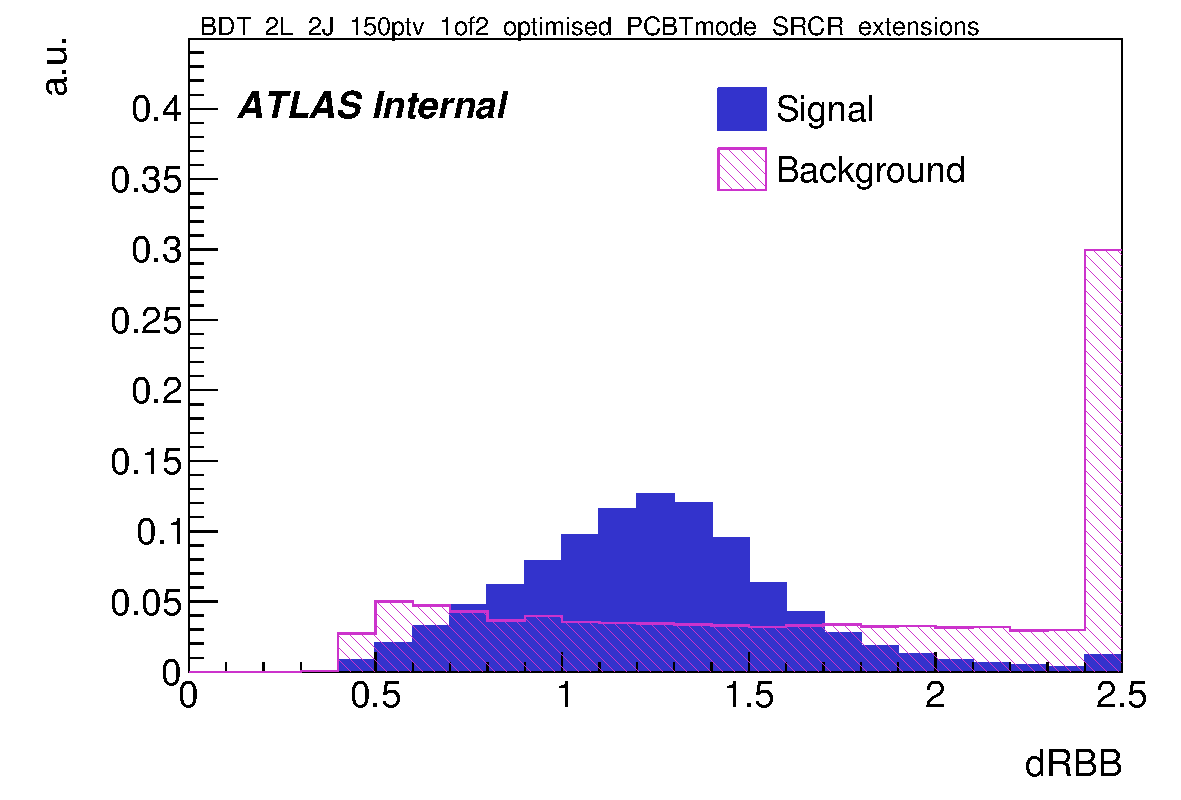
\includegraphics[width=0.33\linewidth]{2-lep-mva/Distr_SignalBackground_dRBB_BDT_2L_2J_150ptv_1of2_optimised_PCBTmode_SRCR_extensions-eps-converted-to}}
    \subfloat[]{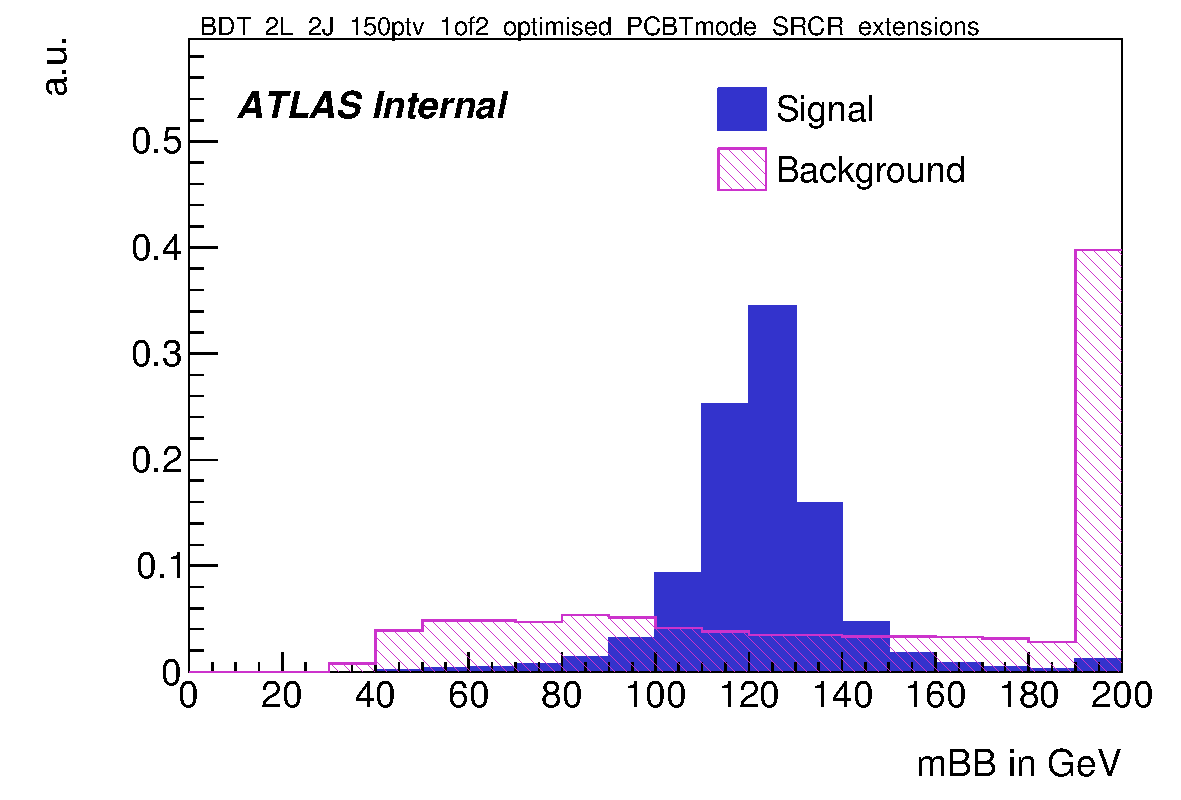
\includegraphics[width=0.33\linewidth]{2-lep-mva/Distr_SignalBackground_mBB_BDT_2L_2J_150ptv_1of2_optimised_PCBTmode_SRCR_extensions-eps-converted-to}}
     \subfloat[]{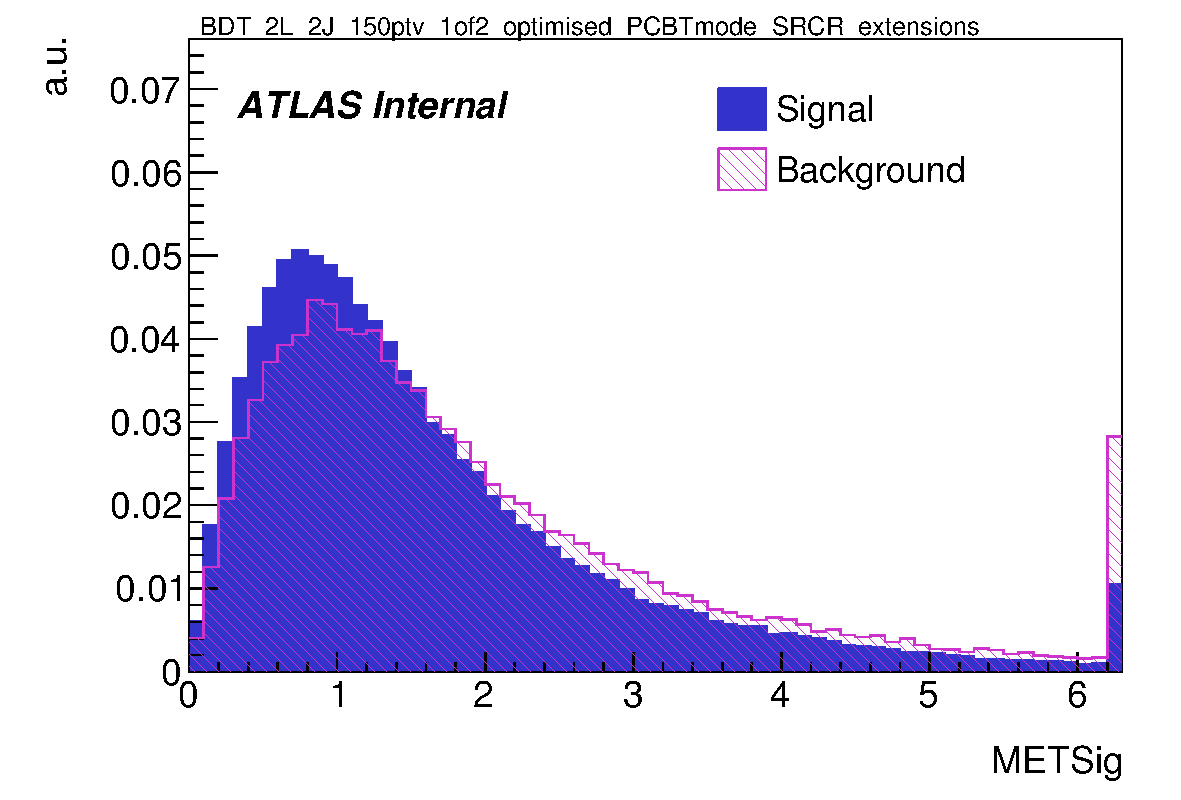
\includegraphics[width=0.33\linewidth]{2-lep-mva/Distr_SignalBackground_METSig_BDT_2L_2J_150ptv_1of2_optimised_PCBTmode_SRCR_extensions-eps-converted-to}}\\
    \subfloat[]{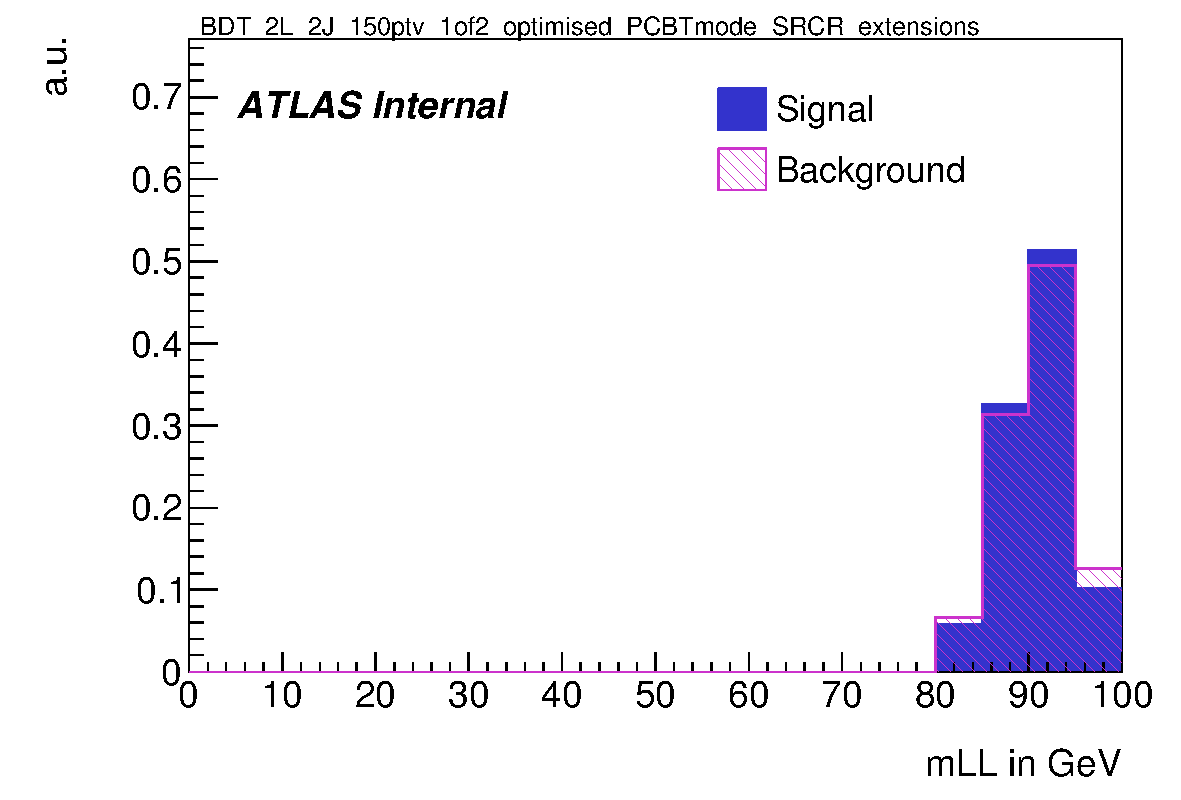
\includegraphics[width=0.33\linewidth]{2-lep-mva/Distr_SignalBackground_mLL_BDT_2L_2J_150ptv_1of2_optimised_PCBTmode_SRCR_extensions-eps-converted-to}}
     \subfloat[]{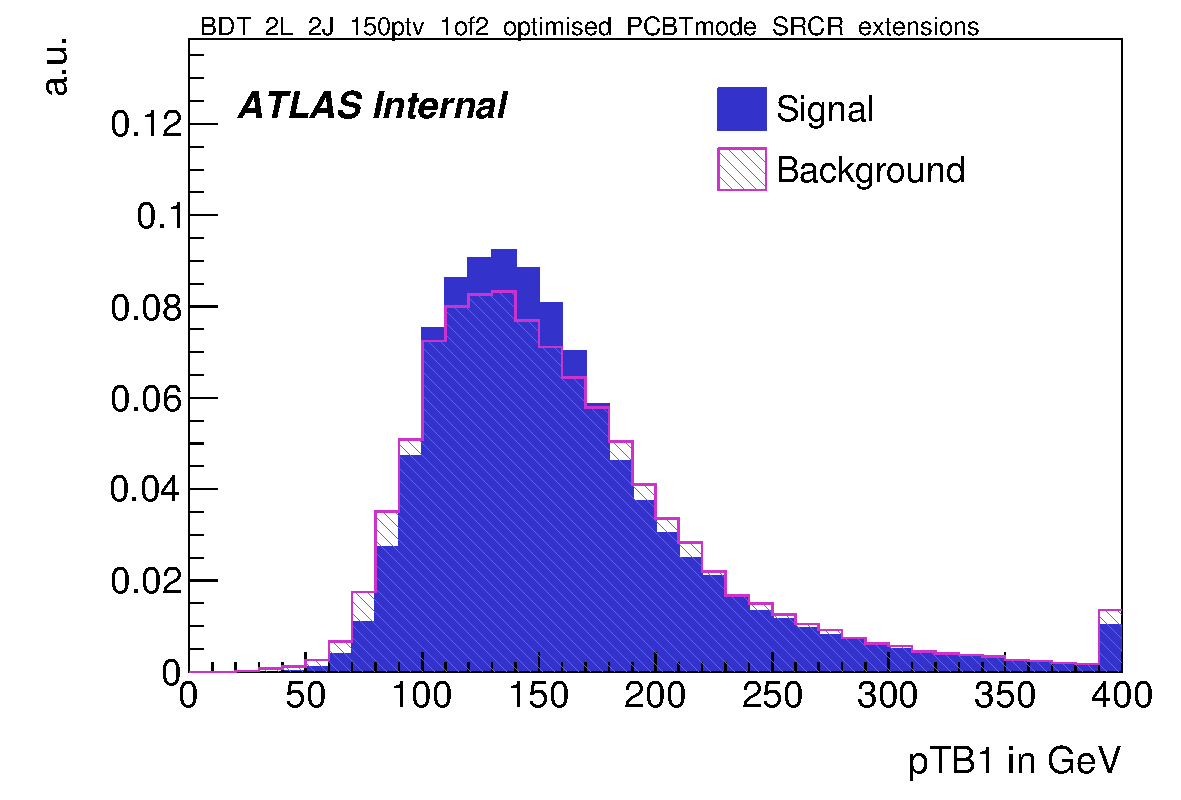
\includegraphics[width=0.33\linewidth]{2-lep-mva/Distr_SignalBackground_pTB1_BDT_2L_2J_150ptv_1of2_optimised_PCBTmode_SRCR_extensions-eps-converted-to}}          
    \subfloat[]{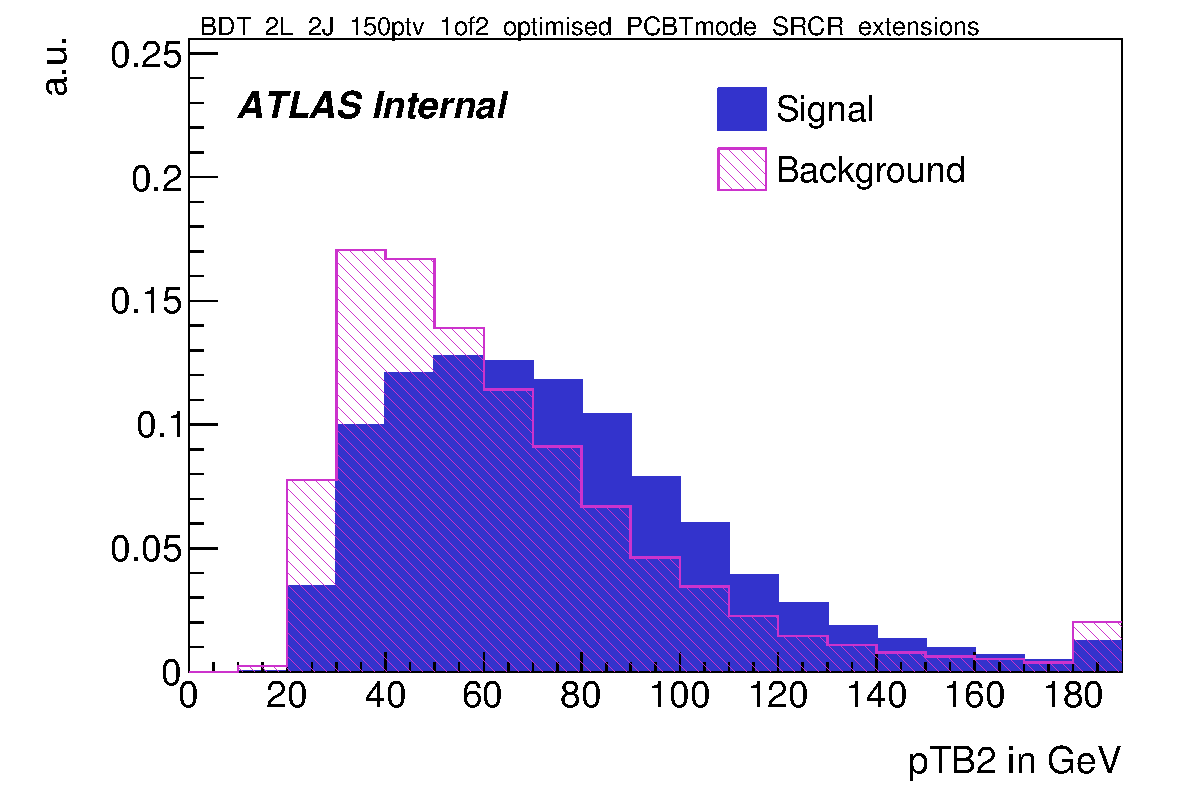
\includegraphics[width=0.33\linewidth]{2-lep-mva/Distr_SignalBackground_pTB2_BDT_2L_2J_150ptv_1of2_optimised_PCBTmode_SRCR_extensions-eps-converted-to}} \\
    \subfloat[]{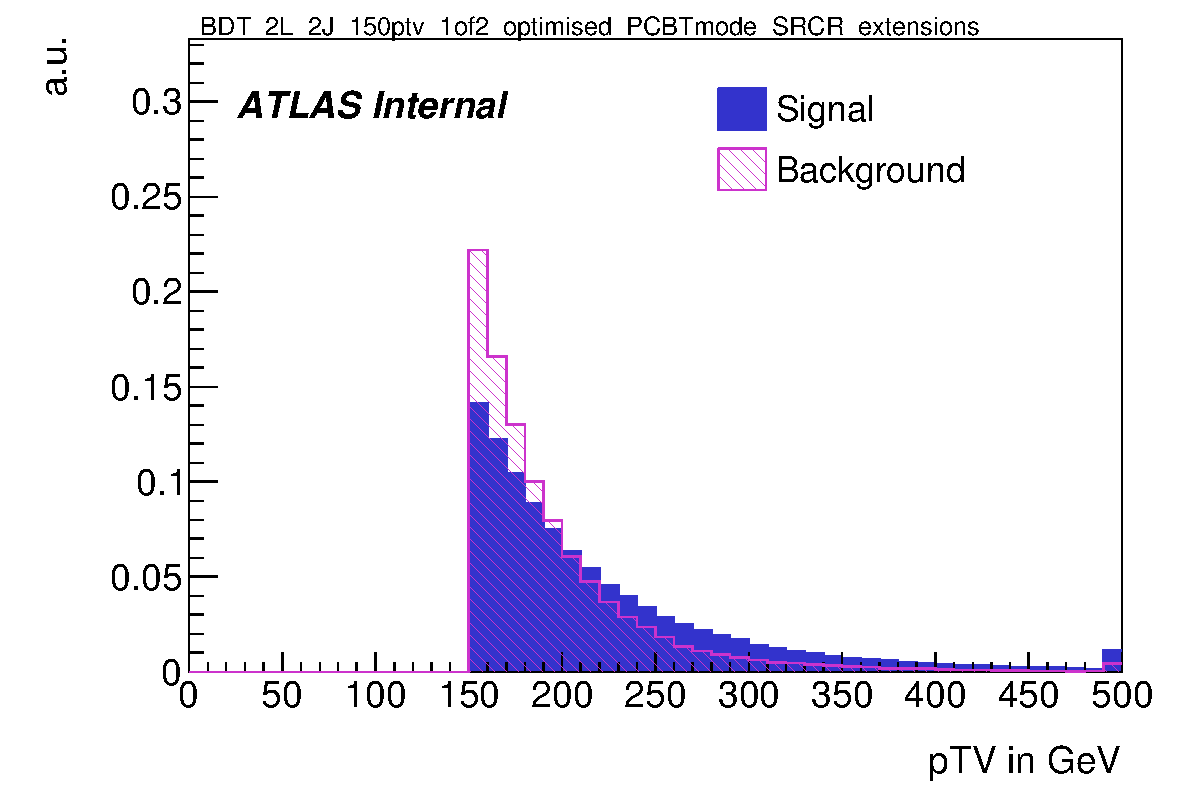
\includegraphics[width=0.33\linewidth]{2-lep-mva/Distr_SignalBackground_pTV_BDT_2L_2J_150ptv_1of2_optimised_PCBTmode_SRCR_extensions-eps-converted-to}}   
    \end{tabular}
    \caption[Inputs to the multi-variate analysis in the 2--lepton 2--jet
    region.]{Inputs to the multi-variate analysis in the 2--lepton 2--jet
      region. Signal events are shown in blue and background events are shown in
      red. The signal and background histograms have been normalised to the same
      area.The distributions only include events with $p_{\mathrm{T}}^{Z}$ > 150
      \GeV.}
    \label{fig:bdtinputs-2lep}
\end{figure}
